\documentclass[11pt,a4paper]{article}

\usepackage[utf8]{inputenc}
\usepackage[T1]{fontenc}
\usepackage[numbers]{natbib}
\usepackage[english]{babel}
\usepackage{geometry}
\usepackage{graphicx}
\usepackage{booktabs}
\usepackage{amsmath}
\usepackage{siunitx}
\usepackage{float}
\usepackage{xcolor}
\usepackage{hyperref}

\geometry{margin=2.3cm}
\graphicspath{{figures/}}
\DeclareSIUnit{\rpm}{rpm}
\sisetup{per-mode=symbol}

\hypersetup{
  colorlinks=true,
  linkcolor=blue!55!black,
  citecolor=blue!55!black,
  urlcolor=blue!55!black
}

\title{\textbf{Modal Analysis of a PETG-CF Fan Housing}\\
\large V5 orientation: base on the \(XY\) plane and height along \(+Z\)}
\author{Numerical study prepared in \texttt{ETUDE\_MODALE\_PETGCF\_COMPOSANTS\_V5\_SOCLE\_XY\_Z}}
\date{15 June 2026}

\begin{document}

\maketitle

\begin{abstract}
This report documents the finite-element modal analysis of a fan housing
intended to be manufactured in PETG-CF. The purpose is to identify the elastic
natural frequencies of the housing and compare them with excitation frequencies
associated with a blade rotational speed close to \SI{2000}{\rpm}. The final V5
model is oriented with the real base resting on the \(XY\) plane and the fan
height along \(+Z\). The mesh is a validated tetrahedral mesh with 95,358 nodes
and 312,777 TETRA4 elements. The housing is modelled as PETG-CF, while the
motor and electronics are represented as localized equivalent masses. The first
elastic mode is found at \SI{49.214}{\hertz}. The rotation frequency at
\SI{2000}{\rpm} is \SI{33.333}{\hertz}, and the five-blade passing frequency is
\SI{166.667}{\hertz}. The first mode is not directly coincident with the 1X
rotation line, and no computed mode is directly coincident with the five-blade
passing line. The third mode, however, is close to the 4X rotational harmonic
and should be monitored in later design iterations.
\end{abstract}

\section{Objective}

The study objective is to evaluate whether the fan housing has natural
frequencies close to the main operating excitations. For a nominal rotational
speed \(N=\SI{2000}{\rpm}\),
\begin{equation}
  f_{\mathrm{rot}} = \frac{N}{60}
  = \SI{33.333}{\hertz}.
\end{equation}
For five blades, the blade passing frequency is
\begin{equation}
  f_{\mathrm{BPF}} = 5 f_{\mathrm{rot}}
  = \SI{166.667}{\hertz}.
\end{equation}
The relevant comparison therefore includes the 1X rotational line, its
harmonics, and the blade passing frequency.

\section{Geometry Preparation}

The original CAD was geometrically valid but poorly suited for a robust
tetrahedral mesh. It contained many small faces and short edges, especially on
the arms. The final mesh-preparation geometry replaced highly detailed arms by
simpler prismatic ribs, removed small non-structural faces, and avoided a small
feature that introduced sliver faces during boolean operations.

\begin{table}[H]
  \centering
  \caption{Topology reduction produced by the mesh-preparation step.}
  \label{tab:cadprep}
  \begin{tabular}{lrrrr}
    \toprule
    Geometry & Faces & Edges & Edges \(<\SI{0.1}{mm}\) & Faces \(<\SI{5}{mm^2}\) \\
    \midrule
    Original CAD & 1450 & 4135 & 2299 & 1175 \\
    Mesh-prepared CAD & 274 & 622 & 5 & 18 \\
    \bottomrule
  \end{tabular}
\end{table}

The final V5 orientation was produced after the modal model was validated. The
real support base was identified and placed on the \(XY\) plane, with the fan
height along \(+Z\). This rigid transformation does not change the modal
physics, but it makes the results easier to inspect and communicate.

\section{Mesh and Material Model}

The mesh was generated with the NETGEN tetrahedral algorithm through
SALOME/SMESH~\cite{salome}. The chosen mesh was retained because it computed
robustly and provided a reasonable model size for repeated Code\_Aster runs.

\begin{table}[H]
  \centering
  \caption{Mesh characteristics.}
  \label{tab:mesh}
  \begin{tabular}{lr}
    \toprule
    Quantity & Value \\
    \midrule
    Element type & TETRA4 \\
    Nodes & 95,358 \\
    Volume elements & 312,777 \\
    Mechanical degrees of freedom & 286,074 \\
    Mesh volume & \SI{704189.190}{mm^3} \\
    \bottomrule
  \end{tabular}
\end{table}

The housing material is an equivalent isotropic PETG-CF. This is an engineering
approximation: a printed PETG-CF part is expected to be anisotropic, and its
actual stiffness depends on print orientation, wall count, infill, temperature,
and inter-layer bonding.

\begin{table}[H]
  \centering
  \caption{Equivalent PETG-CF material properties used in the modal model.}
  \label{tab:material}
  \begin{tabular}{lcc}
    \toprule
    Property & Symbol & Value \\
    \midrule
    Young's modulus & \(E\) & \SI{6000}{MPa} \\
    Poisson ratio & \(\nu\) & 0.35 \\
    Density & \(\rho\) & \(1.30\times10^{-9}\) tonne/mm\(^3\) \\
    \bottomrule
  \end{tabular}
\end{table}

\section{Embedded Masses}

The motor and electronics are not modelled as detailed CAD parts. Instead,
their mass is distributed over two local mesh regions. The stiffness in these
regions remains PETG-CF; only the equivalent density is increased.

\begin{figure}[H]
  \centering
  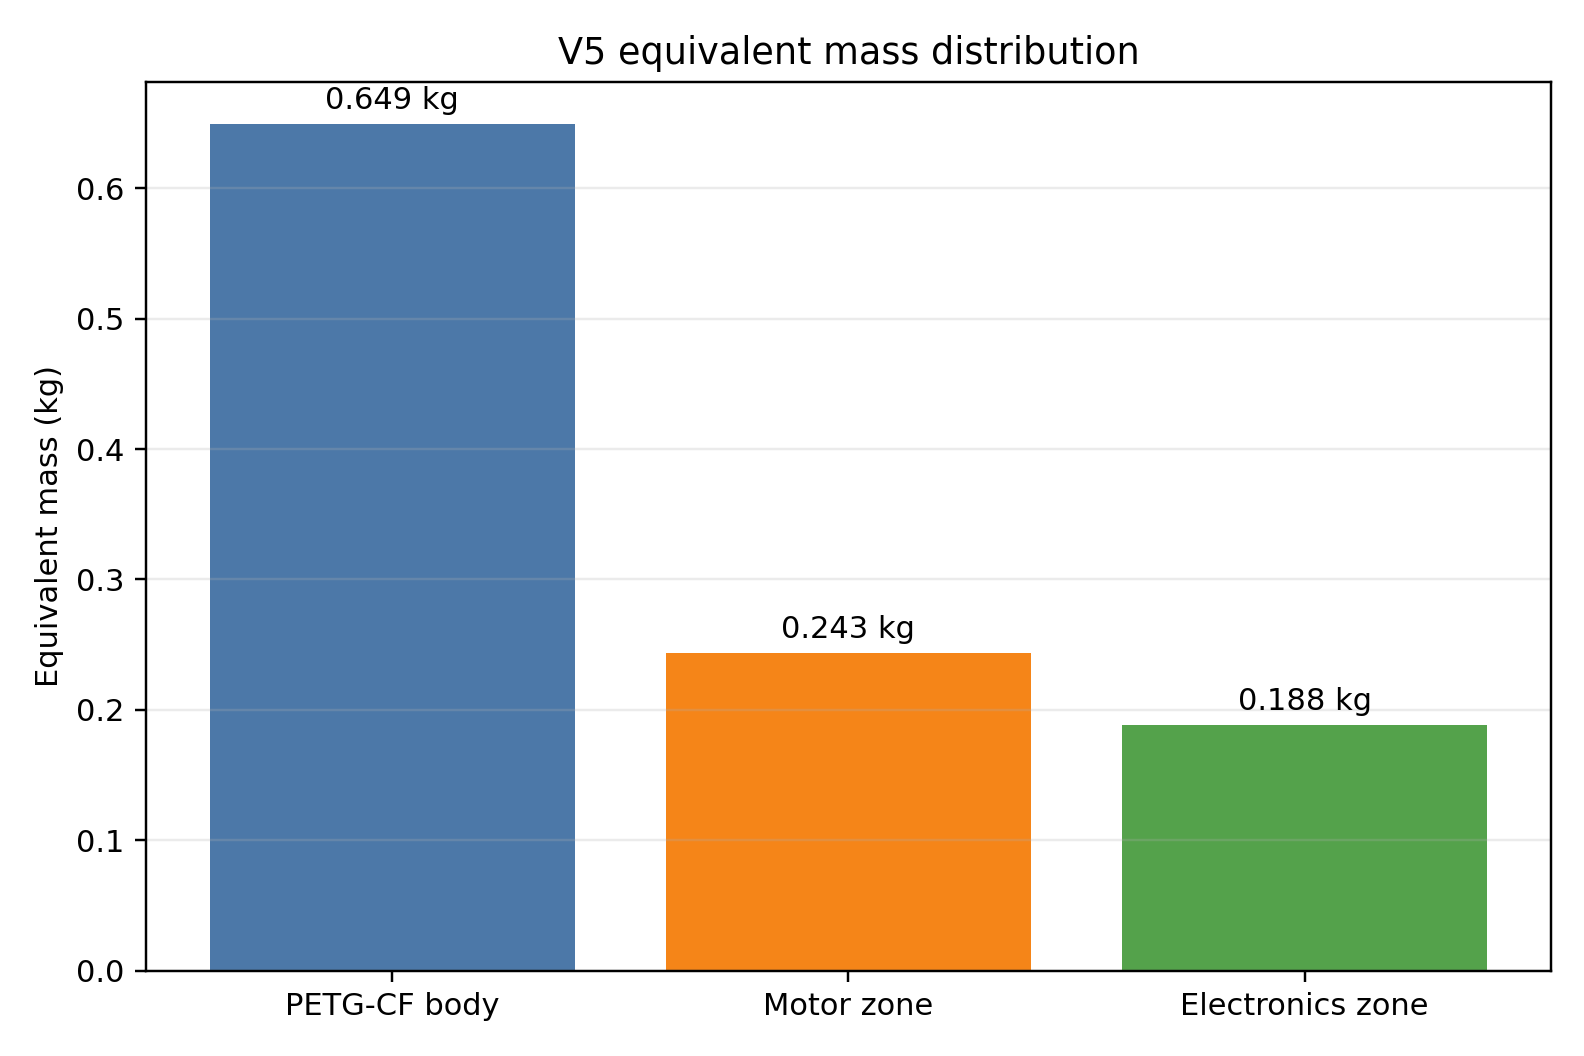
\includegraphics[width=0.74\linewidth]{mass_distribution_en.png}
  \caption{Equivalent mass distribution used in the V5 model.}
  \label{fig:massdist}
\end{figure}

\begin{table}[H]
  \centering
  \caption{Equivalent mass distribution.}
  \label{tab:masses}
  \begin{tabular}{lrrr}
    \toprule
    Zone & Elements & Volume (mm\(^3\)) & Mass (kg) \\
    \midrule
    PETG-CF housing region & 278,034 & 499,125.546 & 0.648863 \\
    Motor region & 23,127 & 117,900.693 & 0.243271 \\
    Electronics base region & 11,616 & 87,162.950 & 0.188312 \\
    \midrule
    Total & 312,777 & 704,189.190 & 1.080446 \\
    \bottomrule
  \end{tabular}
\end{table}

\section{Modal Solver Setup}

The modal problem is solved in Code\_Aster~\cite{codeaster} using a linear 3D
mechanical model in free-free conditions. The stiffness and mass matrices are
assembled and the generalized eigenvalue problem is solved:
\begin{equation}
  K \phi_i = \omega_i^2 M \phi_i.
\end{equation}
The search band is \SIrange{1}{1500}{\hertz}. The six rigid-body modes near
\SI{0}{\hertz} are not listed because the frequency band starts at
\SI{1}{\hertz}. The Code\_Aster run ended with diagnostic \texttt{OK}.

\section{Modal Results}

\begin{table}[H]
  \centering
  \caption{Computed elastic natural frequencies.}
  \label{tab:modes}
  \begin{tabular}{rrr}
    \toprule
    Elastic mode & Aster mode number & Frequency (Hz) \\
    \midrule
     1 &  7 & 49.214 \\
     2 &  8 & 73.181 \\
     3 &  9 & 131.946 \\
     4 & 10 & 250.576 \\
     5 & 11 & 289.925 \\
     6 & 12 & 339.059 \\
     7 & 13 & 377.305 \\
     8 & 14 & 450.782 \\
     9 & 15 & 492.777 \\
    10 & 16 & 522.370 \\
    11 & 17 & 584.026 \\
    12 & 18 & 622.931 \\
    13 & 19 & 643.105 \\
    14 & 20 & 748.567 \\
    15 & 21 & 925.806 \\
    16 & 22 & 1042.368 \\
    17 & 23 & 1137.910 \\
    18 & 24 & 1217.084 \\
    19 & 25 & 1277.192 \\
    20 & 26 & 1393.306 \\
    21 & 27 & 1459.501 \\
    \bottomrule
  \end{tabular}
\end{table}

\begin{figure}[H]
  \centering
  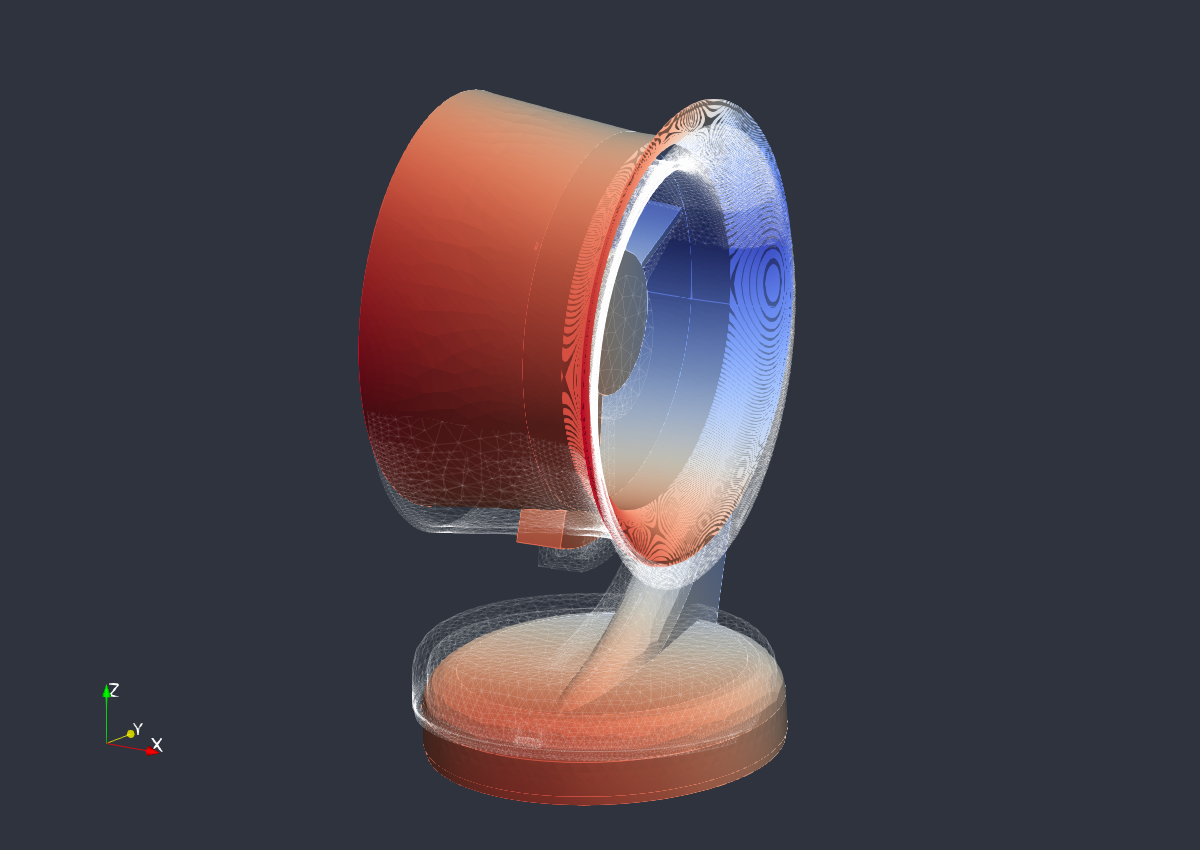
\includegraphics[width=0.92\linewidth]{mode_001_v5_preview.png}
  \caption{First elastic mode at \SI{49.214}{\hertz}. The deformation is
  visually amplified and is not a physical displacement amplitude.}
  \label{fig:mode1}
\end{figure}

\begin{figure}[H]
  \centering
  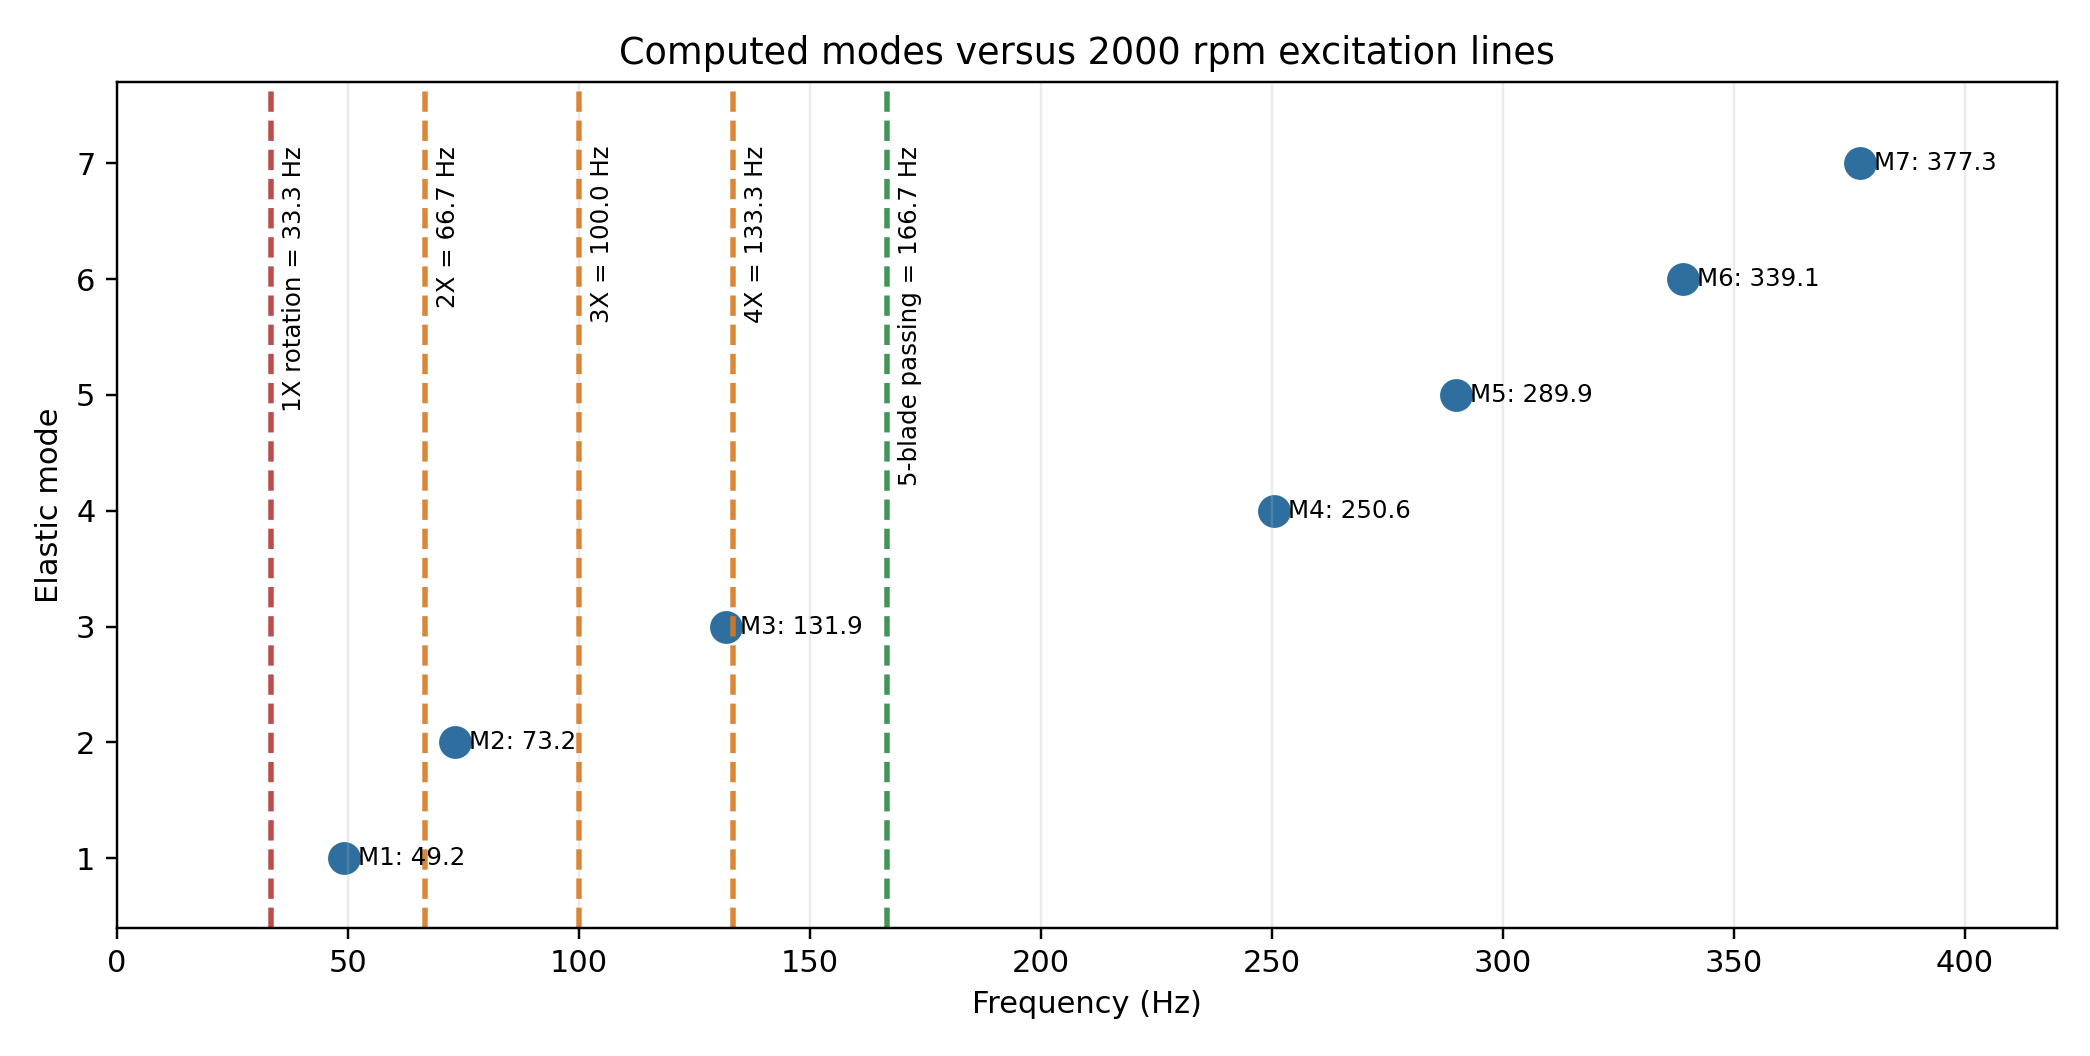
\includegraphics[width=0.98\linewidth]{frequency_excitation_map_en.png}
  \caption{Computed modes compared with excitation lines for
  \SI{2000}{\rpm}.}
  \label{fig:freqmap}
\end{figure}

The first mode is above the 1X rotation line. The third mode at
\SI{131.946}{\hertz} is close to the 4X rotational harmonic at
\SI{133.333}{\hertz}; this is the main frequency proximity observed in the
current free-free model. The five-blade passing frequency at
\SI{166.667}{\hertz} is not directly coincident with a computed natural
frequency.

\section{Mass-Only Estimate for Adding Five Blades}

The blades are not yet included in the finite-element model. A first-order
estimate can be made by assuming that the five blades only add mass and do not
change the structural stiffness:
\begin{equation}
  f_{\mathrm{new}} \approx f_0
  \sqrt{\frac{M_0}{M_0+\Delta M}},
  \label{eq:massonly}
\end{equation}
where \(f_0=\SI{49.214}{\hertz}\), \(M_0=\SI{1.080446}{kg}\), and
\(\Delta M\) is the total blade mass.

\begin{table}[H]
  \centering
  \caption{Mass-only estimate for adding five blades.}
  \label{tab:blades}
  \begin{tabular}{rrrrr}
    \toprule
    Mass per blade (g) & Five blades (kg) & Mode 1 (Hz) & Mode 2 (Hz) & Mode 3 (Hz) \\
    \midrule
     5 & 0.025 & 48.654 & 72.349 & 130.445 \\
    10 & 0.050 & 48.113 & 71.544 & 128.995 \\
    15 & 0.075 & 47.590 & 70.766 & 127.592 \\
    20 & 0.100 & 47.083 & 70.013 & 126.234 \\
    25 & 0.125 & 46.593 & 69.283 & 124.918 \\
    30 & 0.150 & 46.117 & 68.575 & 123.642 \\
    \bottomrule
  \end{tabular}
\end{table}

\begin{figure}[H]
  \centering
  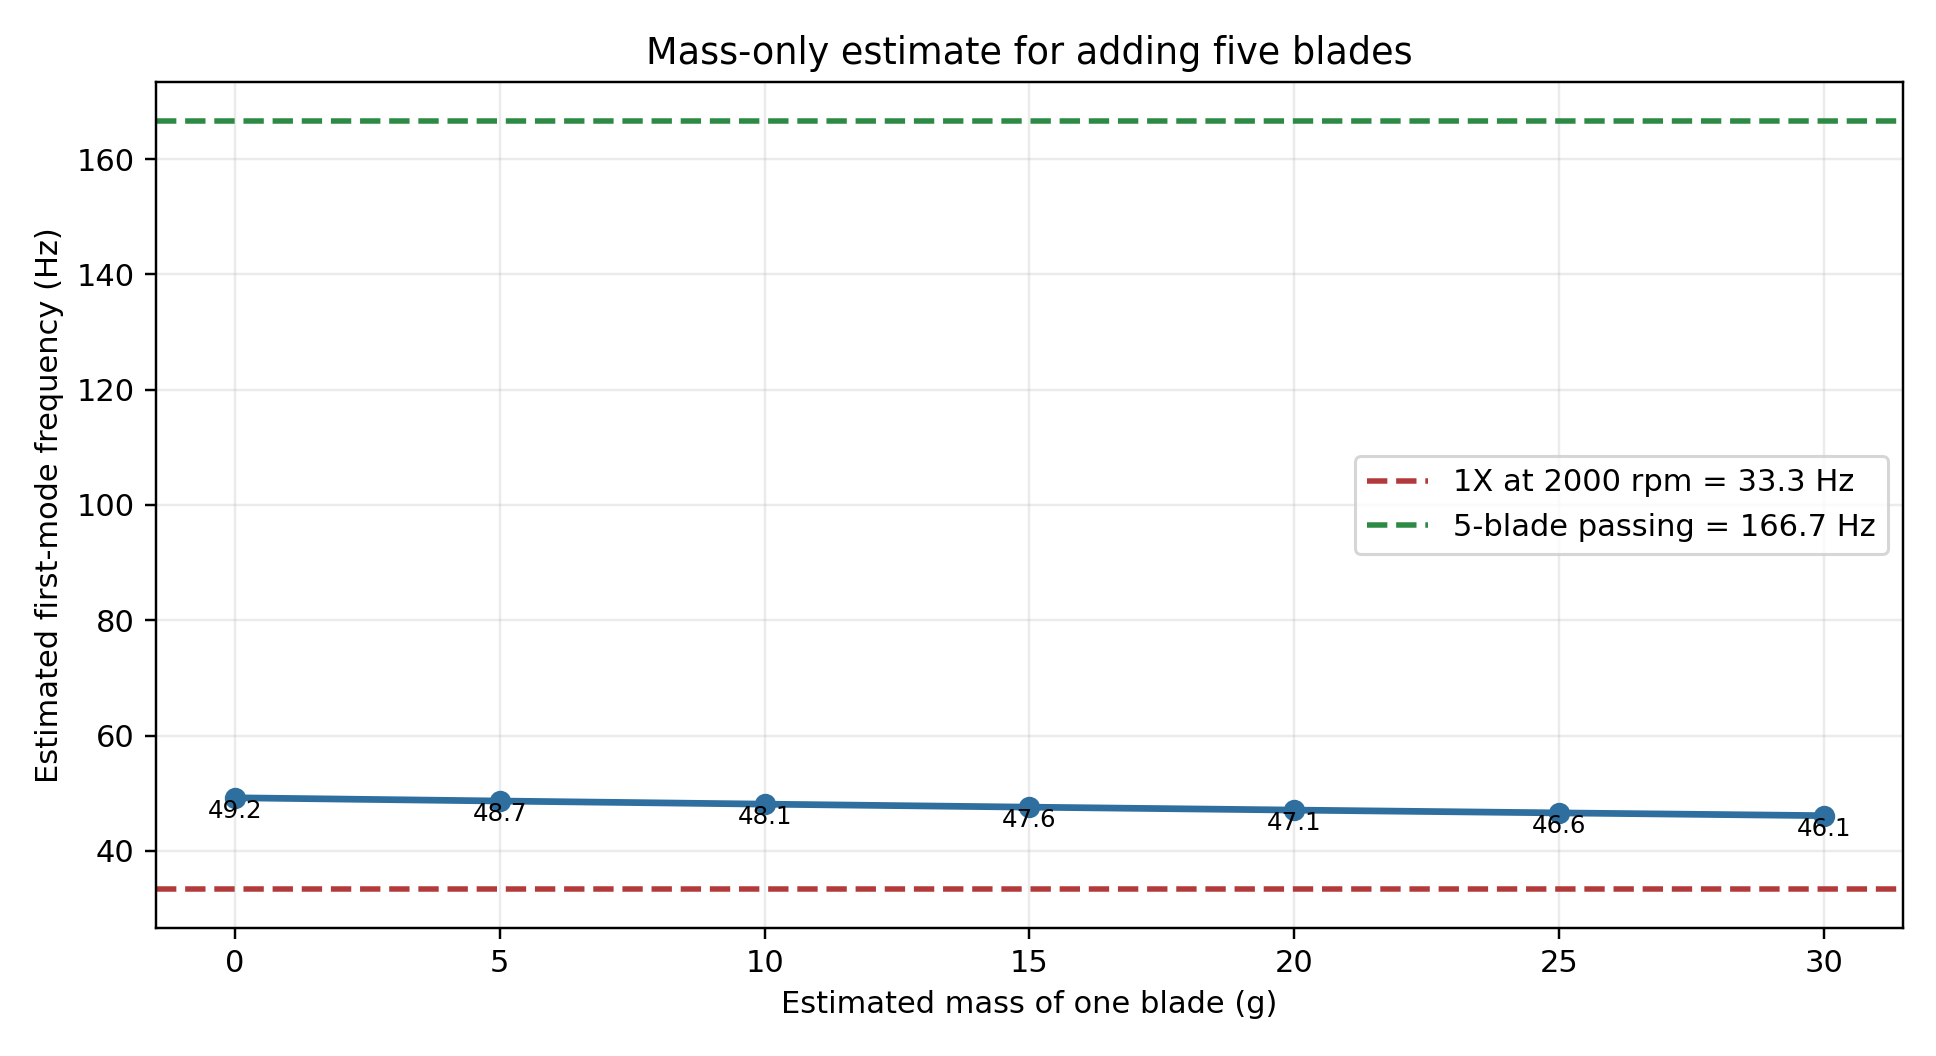
\includegraphics[width=0.88\linewidth]{blade_mass_sensitivity_en.png}
  \caption{Estimated shift of the first mode when five blades are added as
  mass only.}
  \label{fig:blades}
\end{figure}

\section{Effect of a Circular Gasket Under the Base}

Adding a circular gasket under the base is relevant, but it must be represented
by the right physical mechanism. In the present free-free modal model, adding a
gasket without any support condition would have little meaning unless its mass
is included. The important effect of a gasket is usually not its mass but its
compliance and damping at the interface between the fan and the table/support.

Three levels of modelling are possible:
\begin{enumerate}
  \item add the gasket mass only: useful if the gasket is heavy, but usually a
  small effect on frequencies;
  \item model the gasket as distributed elastic supports under the base:
  appropriate for studying how support stiffness shifts the modes;
  \item model a real rubber layer or contact interface: needed for more
  realistic damping and shock behaviour, but requires rubber properties and
  contact assumptions.
\end{enumerate}

For modal analysis, the most useful next step is a supported modal model with
vertical and lateral stiffnesses under the circular base. The expected outcome
is that rigid-body modes disappear, low-frequency supported modes appear, and
some housing modes may shift depending on gasket stiffness. A very soft gasket
can isolate vibration but may introduce low-frequency rocking modes; a very
stiff gasket behaves almost like a hard support.

\section{Drop or Shock Analysis Feasibility}

A table drop is a different problem from a modal analysis. Modal analysis gives
natural frequencies and mode shapes; a drop requires transient dynamics,
contact, and possibly nonlinear material behaviour.

The impact velocity for a drop height \(h\) is approximately
\begin{equation}
  v_0 = \sqrt{2 g h}.
\end{equation}
For example, a \SI{0.8}{m} table drop gives \(v_0\approx\SI{3.96}{m/s}\).
The most important unknown is not only the velocity, but the stopping distance
or contact duration. A short stopping distance produces a high deceleration and
therefore high stresses.

There are two practical modelling routes:
\begin{enumerate}
  \item simplified shock load: impose an equivalent acceleration pulse or
  deceleration level and run a transient or quasi-static check;
  \item nonlinear drop model: include the floor/contact, gasket/contact
  compliance, transient dynamics, and possibly nonlinear PETG-CF behaviour.
\end{enumerate}

The simplified shock model is a good first engineering step. The nonlinear drop
model is more realistic but requires additional data: drop height, impact
orientation, floor stiffness, gasket properties, blade and motor mass/inertia,
and PETG-CF failure criteria.

\section{Limitations}

The present model is a useful design-level modal study, but it is not an
experimental validation. The main limitations are:
\begin{itemize}
  \item PETG-CF is treated as isotropic;
  \item the model is free-free and does not include real mounting stiffness;
  \item blades are not explicitly meshed;
  \item damping is not estimated;
  \item the motor and electronics are represented as distributed equivalent
  masses;
  \item no contact or nonlinear impact behaviour is included.
\end{itemize}

\section{Recommended Next Work}

The most useful next simulations are:
\begin{enumerate}
  \item supported modal analysis with a circular gasket stiffness under the
  base;
  \item sensitivity study versus gasket stiffness and gasket thickness;
  \item mass and inertia representation of the five blades;
  \item simplified shock analysis using an acceleration pulse for a table drop;
  \item experimental tap test or microphone/accelerometer measurement to
  compare real frequencies with the model.
\end{enumerate}

\section{Reproducibility}

The main files are:
\begin{itemize}
  \item Code\_Aster command file:
  \path{03_CODE_ASTER/carter_modal_petgcf_composants_v5_socle_xy_z.comm};
  \item oriented mesh:
  \path{02_MAILLAGE/ventilateur_1_meshprep_socle_xy_z_netgen.med};
  \item modal result:
  \path{04_RESULTATS_PARAVIS/carter_modal_petgcf_composants_v5_socle_xy_z_modes.rmed};
  \item ParaViS state:
  \path{04_RESULTATS_PARAVIS/visualisation_modes_v5_socle_xy_z.pvsm};
  \item vibration GIF:
  \path{04_RESULTATS_PARAVIS/mode_001_49p214Hz_vibration_socle_xy_z.gif}.
\end{itemize}

\bibliographystyle{unsrtnat}
\bibliography{references}

\end{document}
